\begin{sidewaysfigure}
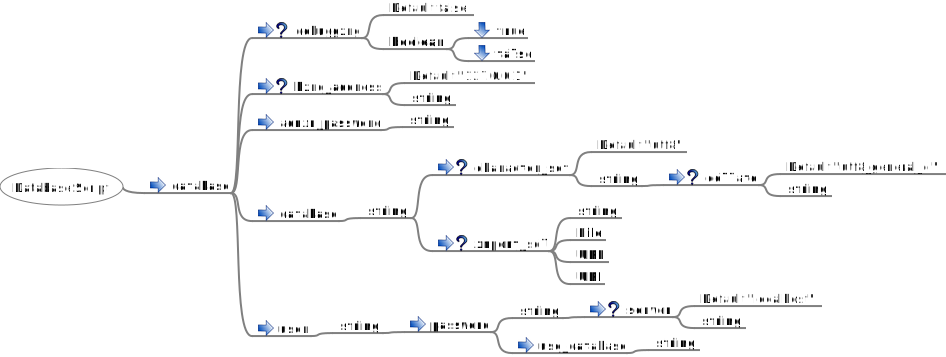
\includegraphics[width=0.9\textwidth]{database_service_script}
\label{fig:database_script_statements}
\caption{Database Script Statements}
\end{sidewaysfigure}

\begin{lstlisting}[style=Java,label=lst:database_ubuntu_profile,caption=Database Example Ubuntu Profile]
profile "ubuntu_10_04", {
    system {
        install_command "export DEBIAN_FRONTEND=noninteractive; /usr/bin/aptitude update && /usr/bin/aptitude install"
    }
    database {
        service "mysql"
        packages "mysql-server"
        configuration_directory "/etc/mysql/conf.d"
        restart_command "/etc/init.d/mysql restart"
    }
}
\end{lstlisting}


\begin{lstlisting}[style=Java,label=lst:database_example_script,caption=Database Example Script]
database {

    // enable debugging output
    debugging true

    // bind the database server to localhost only
    bind_address "127.0.0.1"

    // set the administrator password
    admin_password "mysqladminpassword"

    // add new database with default character set and collate
    database "wordpressdb"

    // add new database
    database "drupal6db" character_set "latin1" collate "latin1_swedish_ci"

    // add new database and import tables
    database "maildb", {
        import_sql "postfixtables.sql"
    }

    // add a new user
    user "test1" password "test1password" server "srv1"

    // add a new user, grand all privileges on database
    user "drupal6" password "drupal6password" server "srv2", {
        use_database "drupal6db"
    }
}
\end{lstlisting}

